% Asset ID: AS2StatisticalDistributionsTikZ-003
% Source: Chapter 6 Statistical Distributions transcript, binomial coefficient explanation
% Related lesson section: Core Theory 8.5 and Worked Examples 3-5
% Purpose: Show how tree/path logic produces the binomial probability formula.

\documentclass[tikz,border=8pt]{standalone}
\usepackage{amsmath}
\usetikzlibrary{positioning, arrows.meta}

\begin{document}
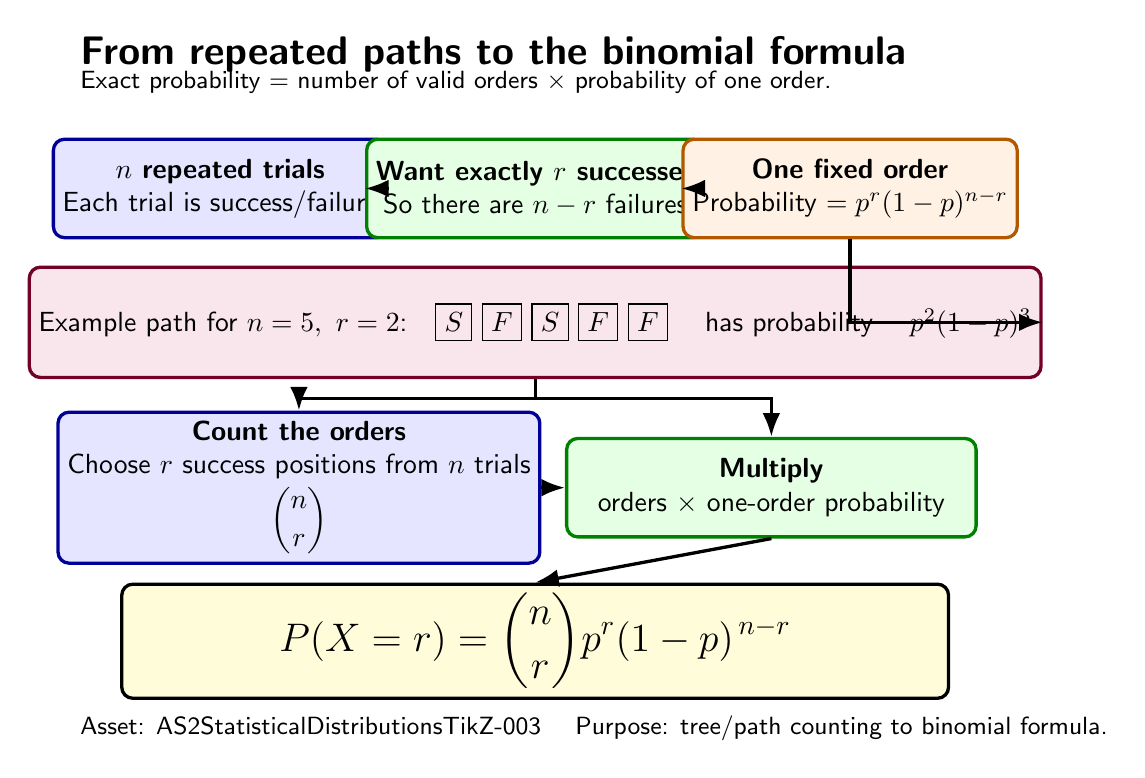
\begin{tikzpicture}[nodebox/.style={draw=black,very thick,rounded corners,fill=white,align=center,font=\sffamily,minimum width=3.9cm,minimum height=1.25cm},bluebox/.style={nodebox,fill=blue!10,draw=blue!60!black},greenbox/.style={nodebox,fill=green!10,draw=green!50!black},orangebox/.style={nodebox,fill=orange!10,draw=orange!70!black},purplebox/.style={nodebox,fill=purple!10,draw=purple!60!black},formula/.style={draw=black,very thick,rounded corners,fill=yellow!15,align=center,font=\Large,minimum width=10.5cm,minimum height=1.1cm},arrow/.style={very thick, -{Latex[length=3mm]}},title/.style={font=\sffamily\bfseries\Large},subtitle/.style={font=\sffamily\small}]
\node[anchor=west, title] at (-5.9,4.2) {From repeated paths to the binomial formula};
\node[anchor=west, subtitle] at (-5.9,3.85) {Exact probability = number of valid orders $\times$ probability of one order.};
\node[bluebox] (trials) at (-4,2.5) {\textbf{$n$ repeated trials}\\Each trial is success/failure};
\node[greenbox] (want) at (0,2.5) {\textbf{Want exactly $r$ successes}\\So there are $n-r$ failures};
\node[orangebox] (onepath) at (4,2.5) {\textbf{One fixed order}\\Probability $=p^r(1-p)^{n-r}$};
\draw[arrow] (trials) -- (want);\draw[arrow] (want) -- (onepath);
\node[purplebox, minimum width=11cm, minimum height=1.4cm] (path) at (0,0.8) {Example path for $n=5,\ r=2$:\quad $\boxed{S}\ \boxed{F}\ \boxed{S}\ \boxed{F}\ \boxed{F}$ \quad has probability \quad $p^2(1-p)^3$};
\draw[arrow] (onepath.south) |- (path.east);
\node[bluebox, minimum width=5.2cm] (choose) at (-3,-1.3) {\textbf{Count the orders}\\Choose $r$ success positions from $n$ trials\\[2pt] $\displaystyle \binom nr$};
\node[greenbox, minimum width=5.2cm] (multiply) at (3,-1.3) {\textbf{Multiply}\\orders $\times$ one-order probability};
\draw[arrow] (path.south) -- ++(0,-0.25) -| (choose.north);\draw[arrow] (path.south) -- ++(0,-0.25) -| (multiply.north);\draw[arrow] (choose) -- (multiply);
\node[formula] (final) at (0,-3.25) {$\displaystyle P(X=r)=\binom nr p^r(1-p)^{\,n-r}$};
\draw[arrow] (multiply.south) -- (final.north);
\node[anchor=west, subtitle] at (-5.9,-4.35) {Asset: AS2StatisticalDistributionsTikZ-003 \quad Purpose: tree/path counting to binomial formula.};
\end{tikzpicture}
\end{document}
